% ============================================================
% Q2: Systemic Sensitivity & Rule Comparison (Rewritten)
% Aligned with Q4 Style (PAGS/Circuit-Breaker Terminology)
% ============================================================
\section{\textbf{Comparative Evaluation of Voting Aggregation Rules and the Judges' Save}  }
\label{sec:q2}

\subsection{The Within-Week Counterfactual Simulation Design }
\label{sec:q2_design}

To isolate the structural properties of aggregation rules from the path dependence of the competition (where one elimination alters all future contestant pools), we adopt a \emph{within-week counterfactual framework}.
For every historical week $(s,t)$, the realized set of active contestants $C_{s,t}$ and the judges' dynamic scoring vector $\mathbf{J}_{s,t}$ are held fixed. The latent fan support is treated not as a point estimate, but as a distribution using the posterior samples $\{\mathbf{v}^{(m)}_{s,t}\}_{m=1}^{M}$ inferred in Model I (Q1), with $M=2000$.
This approach allows for the propagation of uncertainty through the aggregation mechanism, yielding probabilistic estimates of elimination risks under alternative rules rather than deterministic binary outcomes.

\subsection{Mathematical Formalization of Aggregation Regimes}
\label{sec:q2_formalization}

Let $m_{s,t}$ denote the number of contestants to be eliminated in week $(s,t)$. We formalize the two primary historical aggregation rules and the ``Save'' mechanism as distinct mapping functions $E: \mathbb{R}^{|C_{s,t}|} \to 2^{C_{s,t}}$.

\noindent\textbf{Regime A: Percentage Aggregation (Percent)}
\\
The Percentage rule aggregates normalized shares. Let $p^{J}_{i,s,t}$ be the judge-share derived from $\mathbf{J}_{s,t}$, and let $\mathbf v_{s,t}\in\Delta^{|C_{s,t}|-1}$ denote latent \emph{fan vote shares} (not absolute vote counts). The composite score for contestant $i$ is $c_{i,s,t}=p^{J}_{i,s,t}+v_{i,s,t}$.
The elimination set is defined as the subset of size $m_{s,t}$ with the lowest composite scores:
\begin{equation}
    E_{s,t}^{\mathrm{Pct}}(\mathbf{v}_{s,t}) = \mathrm{Bottom}_{m_{s,t}}\left( \mathbf{p}^{J}_{s,t} + \mathbf{v}_{s,t} \right).
\end{equation}

\noindent\textbf{Regime B: Ordinal Rank Aggregation (Rank)}
\\
The Rank rule aggregates ordinal positions. Let $\operatorname{rank}_{\downarrow}(\cdot)$ be the descending rank operator, where rank $1$ denotes the highest score (best performance) and larger ranks indicate worse performance.

Define $r_{i,s,t}^J=\operatorname{rank}_{\downarrow}(J_{i,s,t})$ and $r_{i,s,t}^F=\operatorname{rank}_{\downarrow}(v_{i,s,t})$ as the judge and fan ranks of contestant $i$. The rank-sum disadvantage is $B_{i,s,t}=r_{i,s,t}^J+r_{i,s,t}^F$. Define $\mathrm{Worst}_{m}(\cdot)$ as selecting the indices of the $m$ largest entries (ties broken deterministically). The elimination set corresponds to the $m_{s,t}$ largest rank sums:
\begin{equation}
    E_{s,t}^{\mathrm{Rank}}(\mathbf{v}_{s,t}) = \mathrm{Worst}_{m_{s,t}}\left( \mathbf{r}_{s,t}^J + \mathbf{r}_{s,t}^F(\mathbf{v}_{s,t}) \right).
\end{equation}



\noindent\textbf{Regime C: The Idealized Meritocratic Save (IMS)}
\\
We introduce an \emph{Idealized Meritocratic Save (IMS)} as a \textbf{ceiling benchmark} on how much a save layer \emph{could} correct fan-driven eliminations under purely technical decision-making. Since DWTS is an entertainment program, real judges may deviate from merit; thus IMS is \emph{not} a behavioral model, but an upper bound that brackets the maximum potential technical correction. 

Such deviations can be interpreted as an additive disturbance in the save choice (set to zero here to preserve interpretability and parsimony).


Given a base rule $R\in\{\mathrm{Pct},\mathrm{Rank}\}$, let $\mathbf z^R_{s,t}(\mathbf v)$ denote its baseline decision score vector on week $(s,t)$:
\[
\mathbf z^{\mathrm{Pct}}_{s,t}(\mathbf v)=\mathbf p^J_{s,t}+\mathbf v,\qquad
\mathbf z^{\mathrm{Rank}}_{s,t}(\mathbf v)=\mathbf r^J_{s,t}+\mathbf r^F_{s,t}(\mathbf v),
\]
where larger $\mathbf z^{\mathrm{Rank}}$ indicates worse standing (rank-sum disadvantage).
Define the Bottom-2 set under rule $R$ as $\mathrm{Bottom2}(\mathbf z^R_{s,t}(\mathbf v))$ using the appropriate ordering. IMS then eliminates the weaker technical performer within this bottom tier:
\begin{equation}
E_{s,t}^{R+\mathrm{IMS}}(\mathbf{v}_{s,t}) =
\left\{ \arg\min_{k \in \mathrm{Bottom2}(\mathbf{z}^R_{s,t}(\mathbf{v}_{s,t}))} J_{k,s,t} \right\}.
\end{equation}


\subsection{Uncertainty Propagation and Comparative Metric Formulation }
\label{sec:q2_metrics}

Consistent with the uncertainty propagation in Q1, all comparative metrics are computed as expectations over the posterior draws.

\paragraph{Disagreement Probability ($P_{\mathrm{diff}}$).}
The probability that the two regimes yield different elimination sets:
\begin{equation}
    P_{\mathrm{diff}}(s,t) = \frac{1}{M} \sum_{m=1}^M \mathbf{1}\left\{ E_{s,t}^{\mathrm{Pct}}(\mathbf{v}^{(m)}_{s,t}) \neq E_{s,t}^{\mathrm{Rank}}(\mathbf{v}^{(m)}_{s,t}) \right\}.
\end{equation}

\paragraph{Expected Symmetric Difference ($D_{\mathrm{exp}}$).}
To measure the magnitude of divergence, we compute the expected cardinality of the symmetric difference:
\begin{equation}
    D_{\mathrm{exp}}(s,t) = \mathbb{E}\left[ \left| E_{s,t}^{\mathrm{Pct}} \Delta E_{s,t}^{\mathrm{Rank}} \right| \right].
\end{equation}

\paragraph{Fan Alignment Index (FAI).}
To quantify the bias of a rule $R$ toward audience agency versus technical merit, we define the FAI. Let $i_F^*$ be the fan-bottom contestant and $i_J^*$ be the judge-bottom contestant.
\begin{equation}
    \mathrm{FAI}^R(s,t) = \Pr(i_F^* \in E^R_{s,t}) - \Pr(i_J^* \in E^R_{s,t}).
\end{equation}
$\mathrm{FAI} > 0$ indicates the mechanism is more likely to eliminate the fan-bottom contestant ($i_F^*$), reflecting stronger fan agency in the marginal elimination decision. In contrast, $\mathrm{FAI} < 0$ indicates a technical-correction tendency: the mechanism is more likely to eliminate the judge-bottom contestant ($i_J^*$) even when the fan-bottom differs, thereby reducing purely popularity-driven eliminations.


\paragraph{Global Consistency ($\rho$).}
Beyond binary elimination, we measure the structural alignment of the entire leaderboard using the Spearman rank correlation $\rho_S$ between the rule-implied order and the latent fan preference order.

\subsection{Structural Volatility and Historical Evolution Analysis }
\label{sec:q2_results}

\subsubsection{Aggregated Sensitivity Analysis}
The counterfactual simulation reveals that the choice of aggregation mechanism is non-trivial. Across 264 elimination weeks, the Rank and Percentage rules produce divergent elimination outcomes in \textbf{26.0\%} of cases ($P_{\mathrm{diff}} = 0.260$), with an average symmetric difference of $D_{\mathrm{exp}} = 0.485$.
This confirms that for a quarter of the show's history, the elimination outcome was determined not by performance or popularity but by the mathematical properties of the aggregation formula.

\begin{figure}[H]
    \centering
    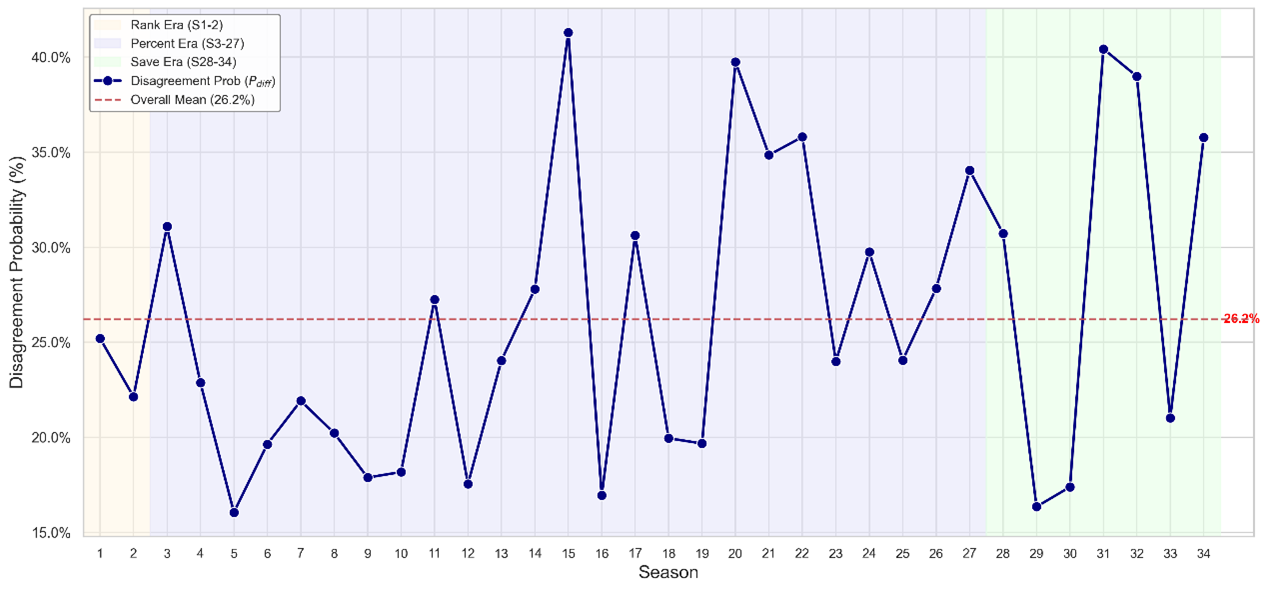
\includegraphics[width=0.55\textwidth]{Q2.4.png}
    \caption{\textbf{Global consistency with fan intent.} Distribution of $\rho$ under Percent (left) and Rank (right); Percent exhibits higher average consistency ($\bar{\rho}=0.765$ vs.\ $0.678$).}
    \label{fig:rho_dist}
\end{figure}

\subsubsection{Era-Dependent Structural Shifts}
Table \ref{tab:phase_metrics} disaggregates these metrics by historical era. Two distinct regimes emerge:

\begin{enumerate}
    \item \textbf{The Agency Regime (S3--27):} Under the Percentage rule, the system exhibits high fan alignment ($\mathrm{FAI}_{\mathrm{Pct}} = 0.277$) and global consistency ($\rho_{\mathrm{Pct}} = 0.765$). This mechanism efficiently translates vote share into survival probability.
    \item \textbf{The Technical Correction Regime (S28--34):} The introduction of the Save mechanism (modeled via IMS) inverts the alignment index ($\mathrm{FAI} < 0$). This is not a numerical anomaly but a quantified structural shift: the two-stage decision process increases the probability that the \emph{technical} bottom ($i_J^*$) is eliminated compared to the \emph{fan} bottom ($i_F^*$).
\end{enumerate}

\begin{table}[H]
    \centering
    \caption{\textbf{Structural Metrics by Historical Era.} Note the inversion of FAI in the Save Era (S28--34), indicating a shift toward meritocratic protection.}
    \label{tab:phase_metrics}
    \small
    \setlength{\tabcolsep}{4pt}
    \begin{tabular}{lccccccc}
        \toprule
        \textbf{Era} & \textbf{Weeks} & \textbf{$P_{\mathrm{diff}}$} & \textbf{$D_{\mathrm{exp}}$} & \textbf{$\mathrm{FAI}_{\mathrm{Pct}}$} & \textbf{$\mathrm{FAI}_{\mathrm{Rank}}$} & \textbf{$\rho_{\mathrm{Pct}}$} & \textbf{$\rho_{\mathrm{Rank}}$} \\
        \midrule
        Rank Era (S1--2)      & 10  & 0.231 & 0.461 & 0.156  & 0.425 & \textbf{0.861}& 0.682 \\
        Percent Era (S3--27)  & 198 & 0.253 & 0.467 & 0.277  & 0.142 & \textbf{0.749}& 0.669 \\
        Save Era (S28--34)    & 56  & \textbf{0.291}& \textbf{0.549}& -0.047 & 0.327 & \textbf{0.804}& 0.710 \\
        \bottomrule
    \end{tabular}
\end{table}

\subsection{Quantification of the IMS Circuit Breaker Effect }
\label{sec:q2_ims}

The IMS baseline isolates the marginal effect of the ``Judges' Save.'' In the 47 weeks where the mechanism reduces to ``Bottom-2 + Re-decision,'' the inclusion of IMS induces a significant negative shift in fan alignment:
\begin{equation}
    \Delta \mathrm{FAI}_{\mathrm{Rank}} = -0.425 \quad \text{and} \quad \Delta \mathrm{FAI}_{\mathrm{Pct}} = -0.055.
\end{equation}
This quantifies the Save mechanism as a \emph{technical circuit breaker}: it systematically overrides fan intent when that intent conflicts with the judges' technical assessment in the bottom tier. The effect is particularly pronounced when superimposed on the Rank mechanism.

\begin{figure}[H]
    \centering
    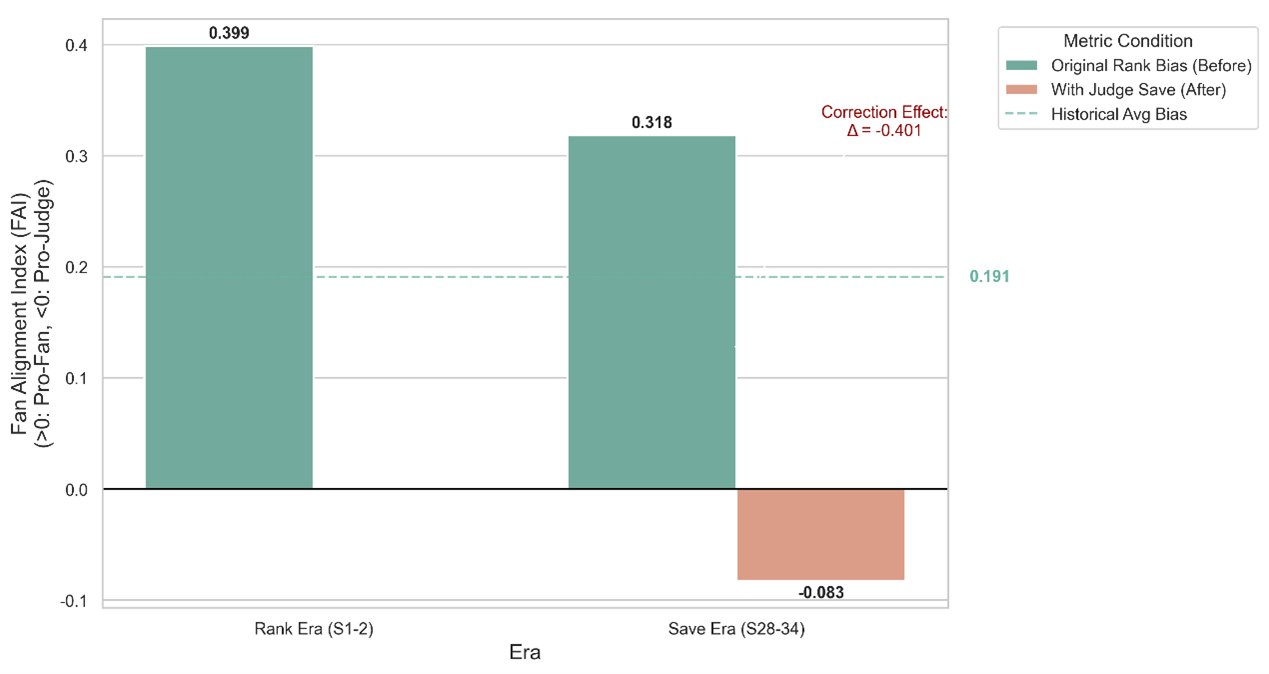
\includegraphics[width=0.72\textwidth]{Q2.3.png}
    \caption{\textbf{Evolution of Fairness (FAI) and Consistency ($\rho$) Across Eras.} The dashed lines represent global historical means. The suppression of FAI in the S28-34 era reflects the active intervention of the Save mechanism.}
    \label{fig:fai_evolution}
\end{figure}

\subsection{Counterfactual Stress Testing of Controversial Profiles }
\label{sec:q2_cases}

To validate the model at the micro-level, we examine specific ``controversial'' contestants—defined as those with high disagreement between judge scores and fan support ($G_i = \mathbb{E}[r^J - r^F]$). We compare their elimination probabilities $p_{\mathrm{elim}}$ in critical weeks under different regimes.

As shown in Table \ref{tab:controversy}, the choice of mechanism is determinant for certain profiles:

\begin{table}[H]
    \centering
    \caption{\textbf{Counterfactual Risk Assessment for High-Variance Profiles.} $\Delta p$ denotes the maximum difference in elimination probability between Rank and Percentage rules in the critical week $t^*$.}
    \label{tab:controversy}
    \footnotesize
    \setlength{\tabcolsep}{3.5pt}
    \renewcommand{\arraystretch}{1.02}
    \begin{tabular}{lcccccc}
        \toprule
        \textbf{Contestant (Season)} & \textbf{Week $t^*$} & \textbf{$p_{\mathrm{elim}}^{\mathrm{Pct}}$} & \textbf{$p_{\mathrm{elim}}^{\mathrm{Rank}}$} & \textbf{$\Delta p$} & \textbf{$p_{\mathrm{elim}}^{\mathrm{Rank+IMS}}$} & \textbf{Divergence $G_i$} \\
        \midrule
        Jerry Rice (S2)      & 3 & \textbf{0.296}& 0.002 & {0.294}& \textbf{0.353}& 1.701 \\
        Billy Ray Cyrus (S4) & 8 & \textbf{0.900}& 0.558 & \textbf{0.341} & 0.822 & 2.088 \\
        Bristol Palin (S11)  & 5 & \textbf{0.124}& 0.087 & 0.036          & \textbf{0.298}& 2.508 \\
        Bobby Bones (S27)    & 1 & \textbf{0.014}& 0.001 & 0.013          & 0.000 & \textbf{3.048}\\
        \bottomrule
    \end{tabular}
\end{table}

\begin{itemize}
    \item \textbf{Type I Divergence (e.g., Jerry Rice, S2):} A massive risk differential ($\Delta p = 0.294$) exists. The Rank mechanism almost guarantees safety ($p=0.002$) due to rank-buffering, whereas Percentage exposes the contestant to significant risk ($p=0.296$).
    \item \textbf{Type II Convergence (e.g., Bobby Bones, S27):} Despite high controversy ($G_i=3.048$), the fan support is so overwhelming that $\Delta p \approx 0$. Here, neither base mechanism suffices to correct the meritocratic deviation, necessitating the stronger ``circuit breaker'' interventions proposed in Section 6 (PAGS).
\end{itemize}




\begin{figure}[H]  % [H] 让图片固定在这里，不再跑到页面顶部
    \centering
    % \makebox 强制让图片在整个文本宽度内居中，消除任何缩进干扰
    \makebox[\textwidth][c]{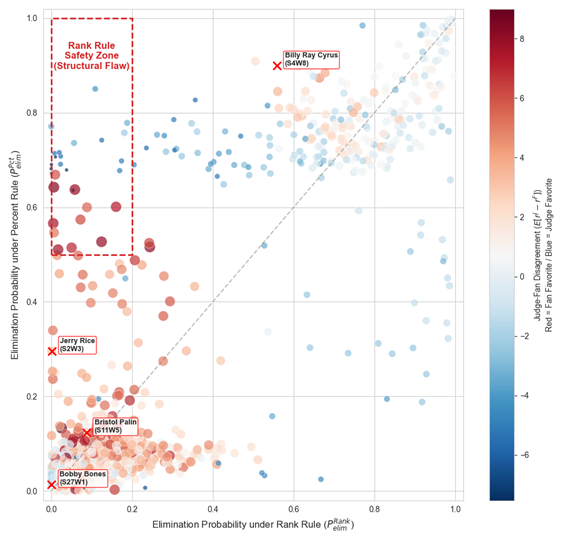
\includegraphics[width=0.48\textwidth]{figures/risk_conflict_map.png}}
   \caption{\textbf{Risk conflict map (Rank vs.\ Percent).} Each point is a contestant-week; x-axis: $p_{\mathrm{elim}}^{\mathrm{Rank}}$, y-axis: $p_{\mathrm{elim}}^{\mathrm{Pct}}$. The highlighted top-left region marks cases that are high-risk under Percent but protected under Rank.}

    \label{fig:risk_conflict_map}
\end{figure}


\subsection{Synthesis of the Merit-Agency Trade-off }
The comparative analysis suggests a fundamental trade-off that informs the design in Section \ref{sec:q4}:
\begin{enumerate}
    \item If the objective is \textbf{Fan Agency (Engagement)}, the Percentage rule is superior ($\rho_{\mathrm{Pct}} > \rho_{\mathrm{Rank}}$), as it preserves the magnitude of popular support.
    \item If the objective is \textbf{Technical Stability}, the Rank mechanism dampens volatility but creates arbitrary safety zones for controversial figures (e.g., Jerry Rice).
    \item To achieve \textbf{Meritocratic Integrity} without sacrificing engagement, a simple rule change is insufficient. The ``Save'' (IMS) provides necessary correction ($\Delta \mathrm{FAI} < 0$), but its opaque application creates consistency issues. This conclusion directly motivates the transparent, parametric guardrails of the PAGS architecture proposed in Q4.
\end{enumerate}